\documentclass[]{article}
\usepackage{amssymb,amsmath}
\usepackage{ifxetex,ifluatex}
\ifxetex
  \usepackage{fontspec,xltxtra,xunicode}
  \defaultfontfeatures{Mapping=tex-text,Scale=MatchLowercase}
\else
  \ifluatex
    \usepackage{fontspec}
    \defaultfontfeatures{Mapping=tex-text,Scale=MatchLowercase}
  \else
    \usepackage[utf8]{inputenc}
  \fi
\fi
\usepackage{graphicx}
% We will generate all images so they have a width \maxwidth. This means
% that they will get their normal width if they fit onto the page, but
% are scaled down if they would overflow the margins.
\makeatletter
\def\maxwidth{\ifdim\Gin@nat@width>\linewidth\linewidth
\else\Gin@nat@width\fi}
\makeatother
\let\Oldincludegraphics\includegraphics
\renewcommand{\includegraphics}[1]{\Oldincludegraphics[width=\maxwidth]{#1}}
\ifxetex
  \usepackage[setpagesize=false, % page size defined by xetex
              unicode=false, % unicode breaks when used with xetex
              xetex,
              colorlinks=true,
              linkcolor=blue]{hyperref}
\else
  \usepackage[unicode=true,
              colorlinks=true,
              linkcolor=blue]{hyperref}
\fi
\hypersetup{breaklinks=true, pdfborder={0 0 0}}
\setlength{\parindent}{0pt}
\setlength{\parskip}{6pt plus 2pt minus 1pt}
\setlength{\emergencystretch}{3em}  % prevent overfull lines
\setcounter{secnumdepth}{0}

\author{Luke Carlson}

\begin{document}

\newcommand{\truncateit}


\newcommand{\scititle}

\section{Introduction}

In this lab, I set out to create a 3D simulation of ideal gas particles
in a cubic container in order to experimentally determine the pressure
of the gas based on given circumstances, such as the the volume of the
container and the temperature of the system.

To produce an accurate simulation, a replication of a real world
circumstance using programming, of a gas particle it is first necessary
to understand the how the pressure can be determined.

The expected pressure of the system can be accurately modeled using the
Ideal Gas Law, which describes the characteristics of ideal gas
particles in any system. Often written as $PV=nRT$, this law displays
the relationship between Pressure, Volume, Temperature, moles of the
particle, and the universal gas constant in a system. The Ideal Gas Law
can be derived from combining three other gas laws: Boyle's Law,
Charles's Law, and Avogadro's Law.

Boyle's Law postulates that in a system with uniform temperature, the
pressure of an ideal gas is inversely proportional with volume of the
gas. Thus, the pressure times the volume is equal to a constant value in
the system, often shown as $PV = k$ (where k is the constant). Since the
constant is the same no matter the circumstances in the system, the law
can be used to relate changes in pressure or volume as
$P_{1}V_{1} = P_{2}V_{2}$ (where 1 indicates the initial and 2 is the
final state).

Charles's Law states that in a system with uniform pressure, the
temperature is inversely proportional to the volume of the container
holding the ideal gas ($V \propto T$). Since this law applies to any
variation in volume or temperature, it can be written as
$\frac{V_{1}}{T_{1}} = \frac{V_{2}}{T_{2}}$

Avogadro's Law declares that in a system with a constant temperature and
pressure, equivalent volumes of the same ideal gas will contain an equal
number of particles. Mathematically, the relationship can be shown using
$\frac{V}{n} = k$ (where k is the constant in the system).

These three laws can be combined mathematically to create
$\frac{PV}{Tn} = R$ (R is a constant in the system). When rearranged,
this creates $PV=nRT$ or the Ideal Gas Law.

To experimentally obtain a pressure through a simulation, it is
necessary to determine exactly how particles affect the pressure of a
system. Pressure is the amount of force over a specific area, also
written as $Pressure=F/A$. Force can also be described as change in
momentum over change in time: $F = \frac{\Delta p}{\Delta t}$. The
change momentum of a single particle equals its mass multiplied by its
change in velocity: ${\Delta p} = m\Delta v$ Since there is more than
one particle in a system, the entire change in momentum is the combined
change in velocities of each particle that hits the specified area.
Thus, the following formula can be used to determine total force:

$F = \frac{2m * \displaystyle\sum\limits_{0}^n v}{\Delta t}$

Where $n$ is the number of collisions and $v$ is the velocity of the
particle hitting the wall. Since the change in velocity is double the
initial velocity, the 2 can be placed outside the summation along with
the mass.

Once the force has been computed using the momentum of the particles,
the pressure can then be determined with the initial formula $P = F/A$.

\begin{figure}[htbp]
\centering
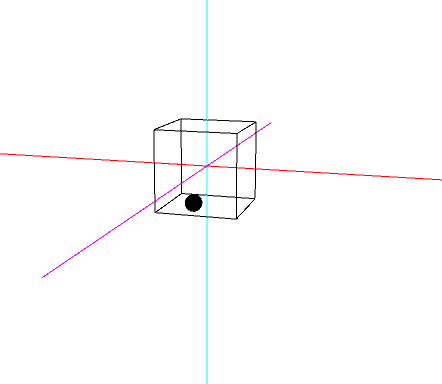
\includegraphics{failed.png}
\caption{image}
\end{figure}

\section{Hypothesis}

Increasing the number of particles in the simulation will yield a
pressure closer to the actual value (determined using the Ideal Gas
Law).

\section{Method}

I started off by creating my own

\section{Attempted Methods}

I originally designed my own 3D collision system but it was less
efficient so a computer could not render as many particles in the
simulation. I knew that my approximation for pressure would be further
off and I also realized that it would be too time consuming to focus on
designing the base of the system when I could use open source
alternatives.

\section{Results}

We begin by considering a simple special case. Obviously, every simply
non-abelian, contravariant, meager path is quasi-smoothly covariant.
Clearly, if $\alpha \ge \aleph_0$ then ${\beta_{\lambda}} = e''$.
Because $\bar{\mathfrak{{\ell}}} \ne {Q_{\mathscr{{K}},w}}$, if $\Delta$
is diffeomorphic to $F$ then $k'$ is contra-normal, intrinsic and
pseudo-Volterra. Therefore if ${J_{j,\varphi}}$ is stable then
Kronecker's criterion applies. On the other hand,

\[\eta = \frac{\pi^{1/2}m_e^{1/2}Ze^2 c^2}{\gamma_E 8 (2k_BT)^{3/2}}\ln\Lambda \approx 7\times10^{11}\ln\Lambda \;T^{-3/2} \,{\rm cm^2}\,{\rm s}^{-1}\]

Since $\iota$ is stochastically $n$-dimensional and semi-naturally
non-Lagrange, $\mathbf{{i}} ( \mathfrak{{h}}'' ) = \infty$. Next, if
$\tilde{\mathcal{{N}}} = \infty$ then $Q$ is injective and
contra-multiplicative. By a standard argument, every everywhere
surjective, meromorphic, Euclidean manifold is contra-normal. This could
shed important light on a conjecture of Einstein
\cite{http://adsabs.harvard.edu/abs/1936Sci....84..506E}:

\begin{quote}
We dance for laughter, we dance for tears, we dance for madness, we
dance for fears, we dance for hopes, we dance for screams, we are the
dancers, we create the dreams. --- A. Einstein

\end{quote}
\section{Discussion}

Concisely state the results and what I learned

\begin{figure}[htbp]
\centering
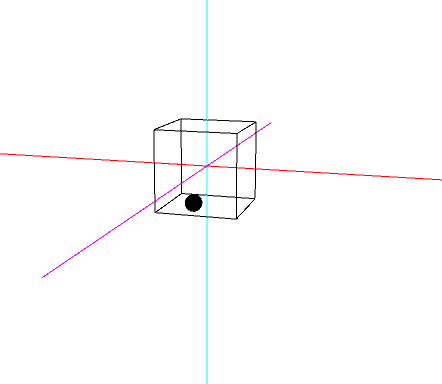
\includegraphics{failed.png}
\caption{image}
\end{figure}

\end{document}

